\documentclass{article}%
\usepackage[T1]{fontenc}%
\usepackage[utf8]{inputenc}%
\usepackage{lmodern}%
\usepackage{textcomp}%
\usepackage{lastpage}%
\usepackage{geometry}%
\geometry{margin=0.5in,headheight=10pt,footskip=0.2in,tmargin=0.5in,bmargin=0.5in}%
\usepackage{graphicx}%
\usepackage{float}%
\usepackage{booktabs}%
\usepackage{hyperref}%
\usepackage{caption}%
\usepackage{subcaption}%
\usepackage{ragged2e}%
%
\title{ML Raport}%
\author{AutoPrep}%
\date{\today}%
%
\begin{document}%
\normalsize%
\maketitle%

    \begin{abstract}
    This raport has been generated with AutoPrep.
    \end{abstract}
    %
\tableofcontents%
\newpage%
\section{Overview}%
\label{sec:Overview}%

%
\subsection{System}%
\label{subsec:System}%

%


\begin{table}[H]%
\begin{center}%
\renewcommand{\arraystretch}{1.5}%
\begin{tabular}{l l}%
\hline%
System&Darwin\\%
Machine&arm64\\%
Processor&arm\\%
Architecture&64bit\\%
Python Version&3.10.5\\%
Physical Cores&8\\%
Logical Cores&8\\%
CPU Frequency (MHz)&3204\\%
Total RAM (GB)&16.00\\%
Available RAM (GB)&4.57\\%
Total Disk Space (GB)&228.27\\%
Free Disk Space (GB)&8.06\\%
\hline%
\end{tabular}%
\end{center}%
\caption{System overview.}%
\end{table}

%
\subsection{Dataset}%
\label{subsec:Dataset}%

%
Table~\ref{tab:dataset_summary} %
presents an overview of the dataset including the number of samples, features, and their types.%


\begin{table}[H]%
\begin{center}%
\renewcommand{\arraystretch}{1.5}%
\begin{tabular}{l l}%
\hline%
Number of samples&227\\%
Number of features&9\\%
Number of numerical features&9\\%
Number of categorical features&0\\%
\hline%
\end{tabular}%
\end{center}%
\caption{Dataset Summary.}%
\label{tab:dataset_summary}%
\end{table}

%
Table~\ref{tab:missing_values} %
presents the distribution of missing values in the dataset.%


\begin{table}[H]%
\begin{center}%
\renewcommand{\arraystretch}{1.5}%
\begin{tabular}{l l l}%
\hline%
\textbf{classgit}&\textbf{number of observations}&\textbf{Percentage}\\%
\hline%
P85&0&0.00\\%
P75&0&0.00\\%
RMT85&0&0.00\\%
CS82&0&0.00\\%
SS82&0&0.00\\%
S82&0&0.00\\%
ME84&0&0.00\\%
REV84&0&0.00\\%
REG&0&0.00\\%
\hline%
\end{tabular}%
\end{center}%
\caption{Missing values distribution.}%
\label{tab:missing_values}%
\end{table}

%
Table~\ref{tab:features_dtypes} %
presents the description of features in the dataset.%


\begin{table}[H]%
\begin{center}%
\renewcommand{\arraystretch}{1.5}%
\begin{tabular}{l l l l}%
\hline%
\textbf{class}&\textbf{type}&\textbf{dtype}&\textbf{space usage}\\%
\hline%
P85&numerical&int64&3.6 kB\\%
P75&numerical&int64&3.6 kB\\%
RMT85&numerical&int64&3.6 kB\\%
CS82&numerical&uint8&2.0 kB\\%
SS82&numerical&uint8&2.0 kB\\%
S82&numerical&uint8&2.0 kB\\%
ME84&numerical&int64&3.6 kB\\%
REV84&numerical&int64&3.6 kB\\%
REG&numerical&uint8&2.0 kB\\%
\hline%
\end{tabular}%
\end{center}%
\caption{Features dtypes description.}%
\label{tab:features_dtypes}%
\end{table}

%
Table~\ref{tab:numerical_features} %
presents the description of numerical features in the dataset.%


\begin{table}[H]%
\begin{center}%
\renewcommand{\arraystretch}{1.5}%
\begin{tabular}{l l l l l l l l l}%
\hline%
\textbf{index}&\textbf{count}&\textbf{mean}&\textbf{std}&\textbf{min}&\textbf{25\%}&\textbf{50\%}&\textbf{75\%}&\textbf{max}\\%
\hline%
P85&227.00&29.99&56.17&3.00&10.00&16.00&30.00&653.00\\%
P75&227.00&29.52&57.77&4.00&10.00&15.00&28.00&671.00\\%
RMT85&227.00&254.51&657.60&21.00&66.50&118.00&229.50&6720.00\\%
CS82&227.00&9.18&4.98&1.00&6.00&8.00&11.00&34.00\\%
SS82&227.00&21.95&7.23&8.00&17.00&21.00&27.00&46.00\\%
S82&227.00&47.15&10.57&31.00&41.00&45.00&49.00&101.00\\%
ME84&227.00&1842.41&4685.06&173.00&480.50&839.00&1580.50&47074.00\\%
REV84&227.00&3048.31&5125.17&347.00&1134.50&1828.00&3174.00&59877.00\\%
REG&227.00&4.33&2.08&1.00&2.00&4.00&6.00&8.00\\%
\hline%
\end{tabular}%
\end{center}%
\caption{Numerical features description.}%
\label{tab:numerical_features}%
\end{table}

%
\section{Eda}%
\label{sec:Eda}%

%
This part of the report provides basic insides to the data and the informations it holds..%
\subsection{Target variable and missing values}%
\label{subsec:Targetvariableandmissingvalues}%

%
Figure~\ref{Target distribution.} %
 shows the distribution of the target variable.%


\begin{figure}[H]%
\centering%
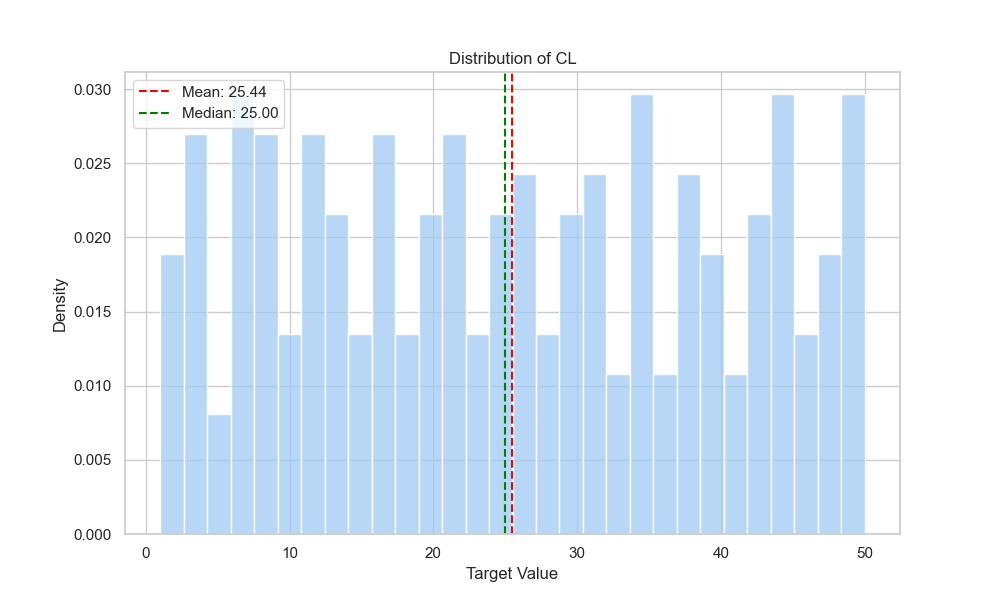
\includegraphics[width=0.9\textwidth]{/Users/julia/Desktop/semestr-5/automl/AutoPrep/examples/raport/raport/charts/target_distribution_regression.png}%
\caption{Target distribution.}%
\label{Target distribution.}%
\end{figure}

%
\subsection{EDA for numerical features}%
\label{subsec:EDAfornumericalfeatures}%

%
The distribution of numerical features is presented on histogram(s) below.%


\begin{figure}[H]%
\centering%
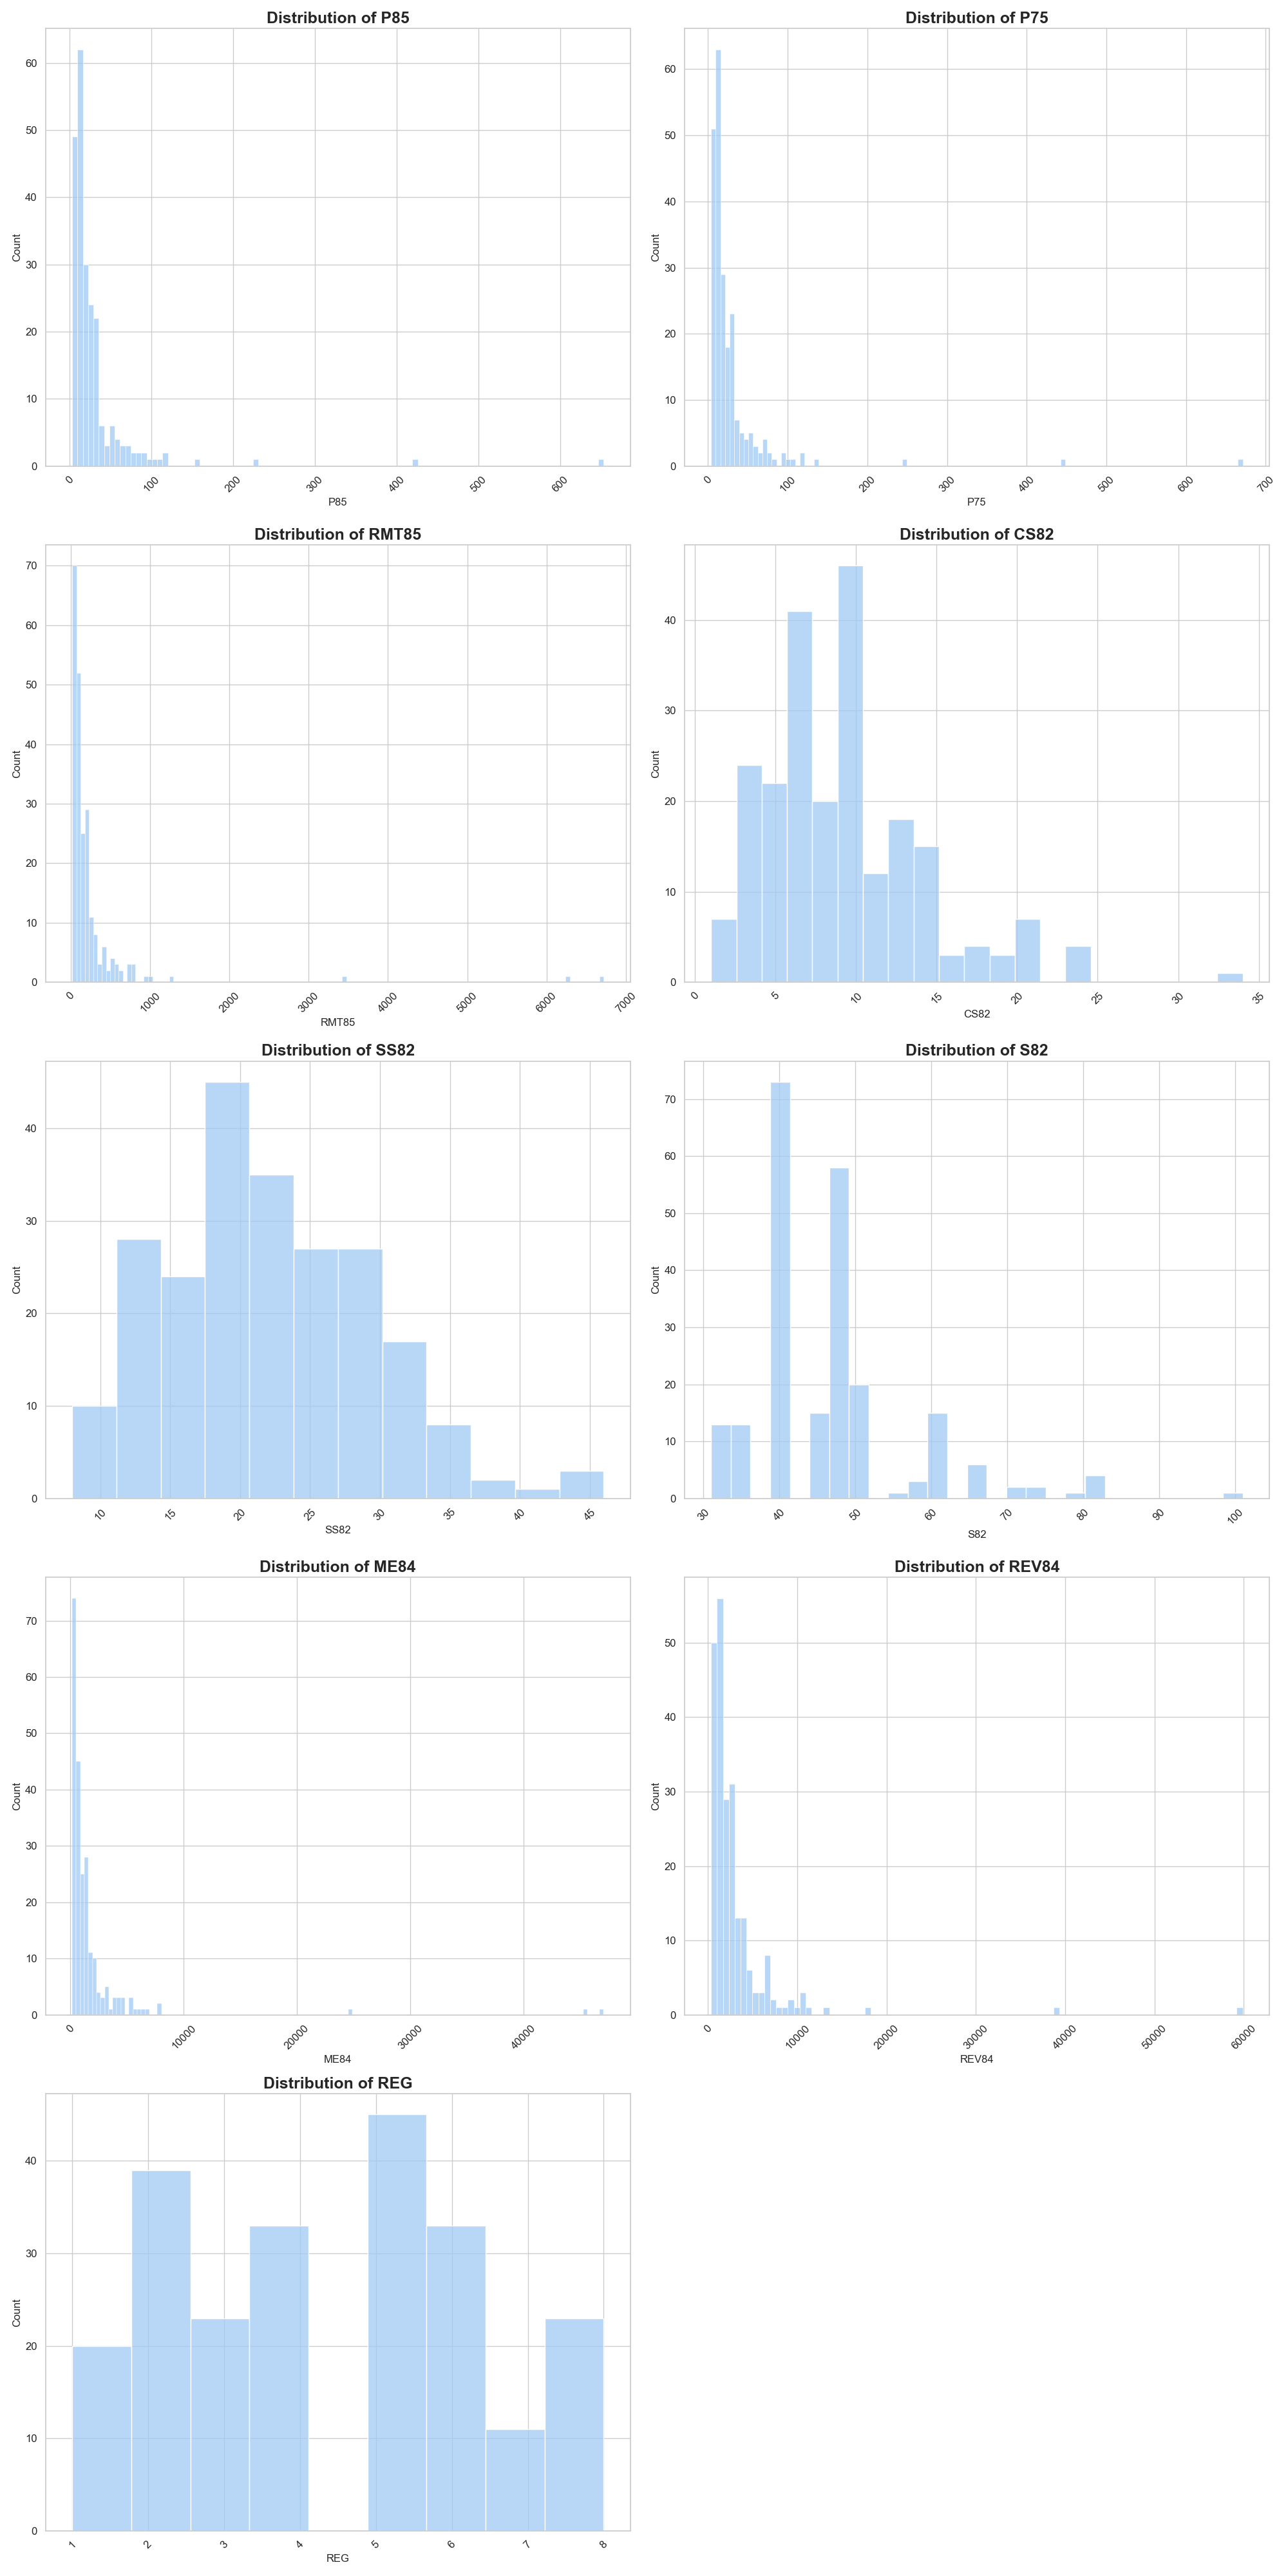
\includegraphics[width=0.9\textwidth]{/Users/julia/Desktop/semestr-5/automl/AutoPrep/examples/raport/raport/charts/numerical_distribution_page_1.png}%
\caption{Numerical Features Distribution {-} Page 1}%
\label{Numerical Features Distribution - Page 1}%
\end{figure}

%


\begin{figure}[H]%
\centering%
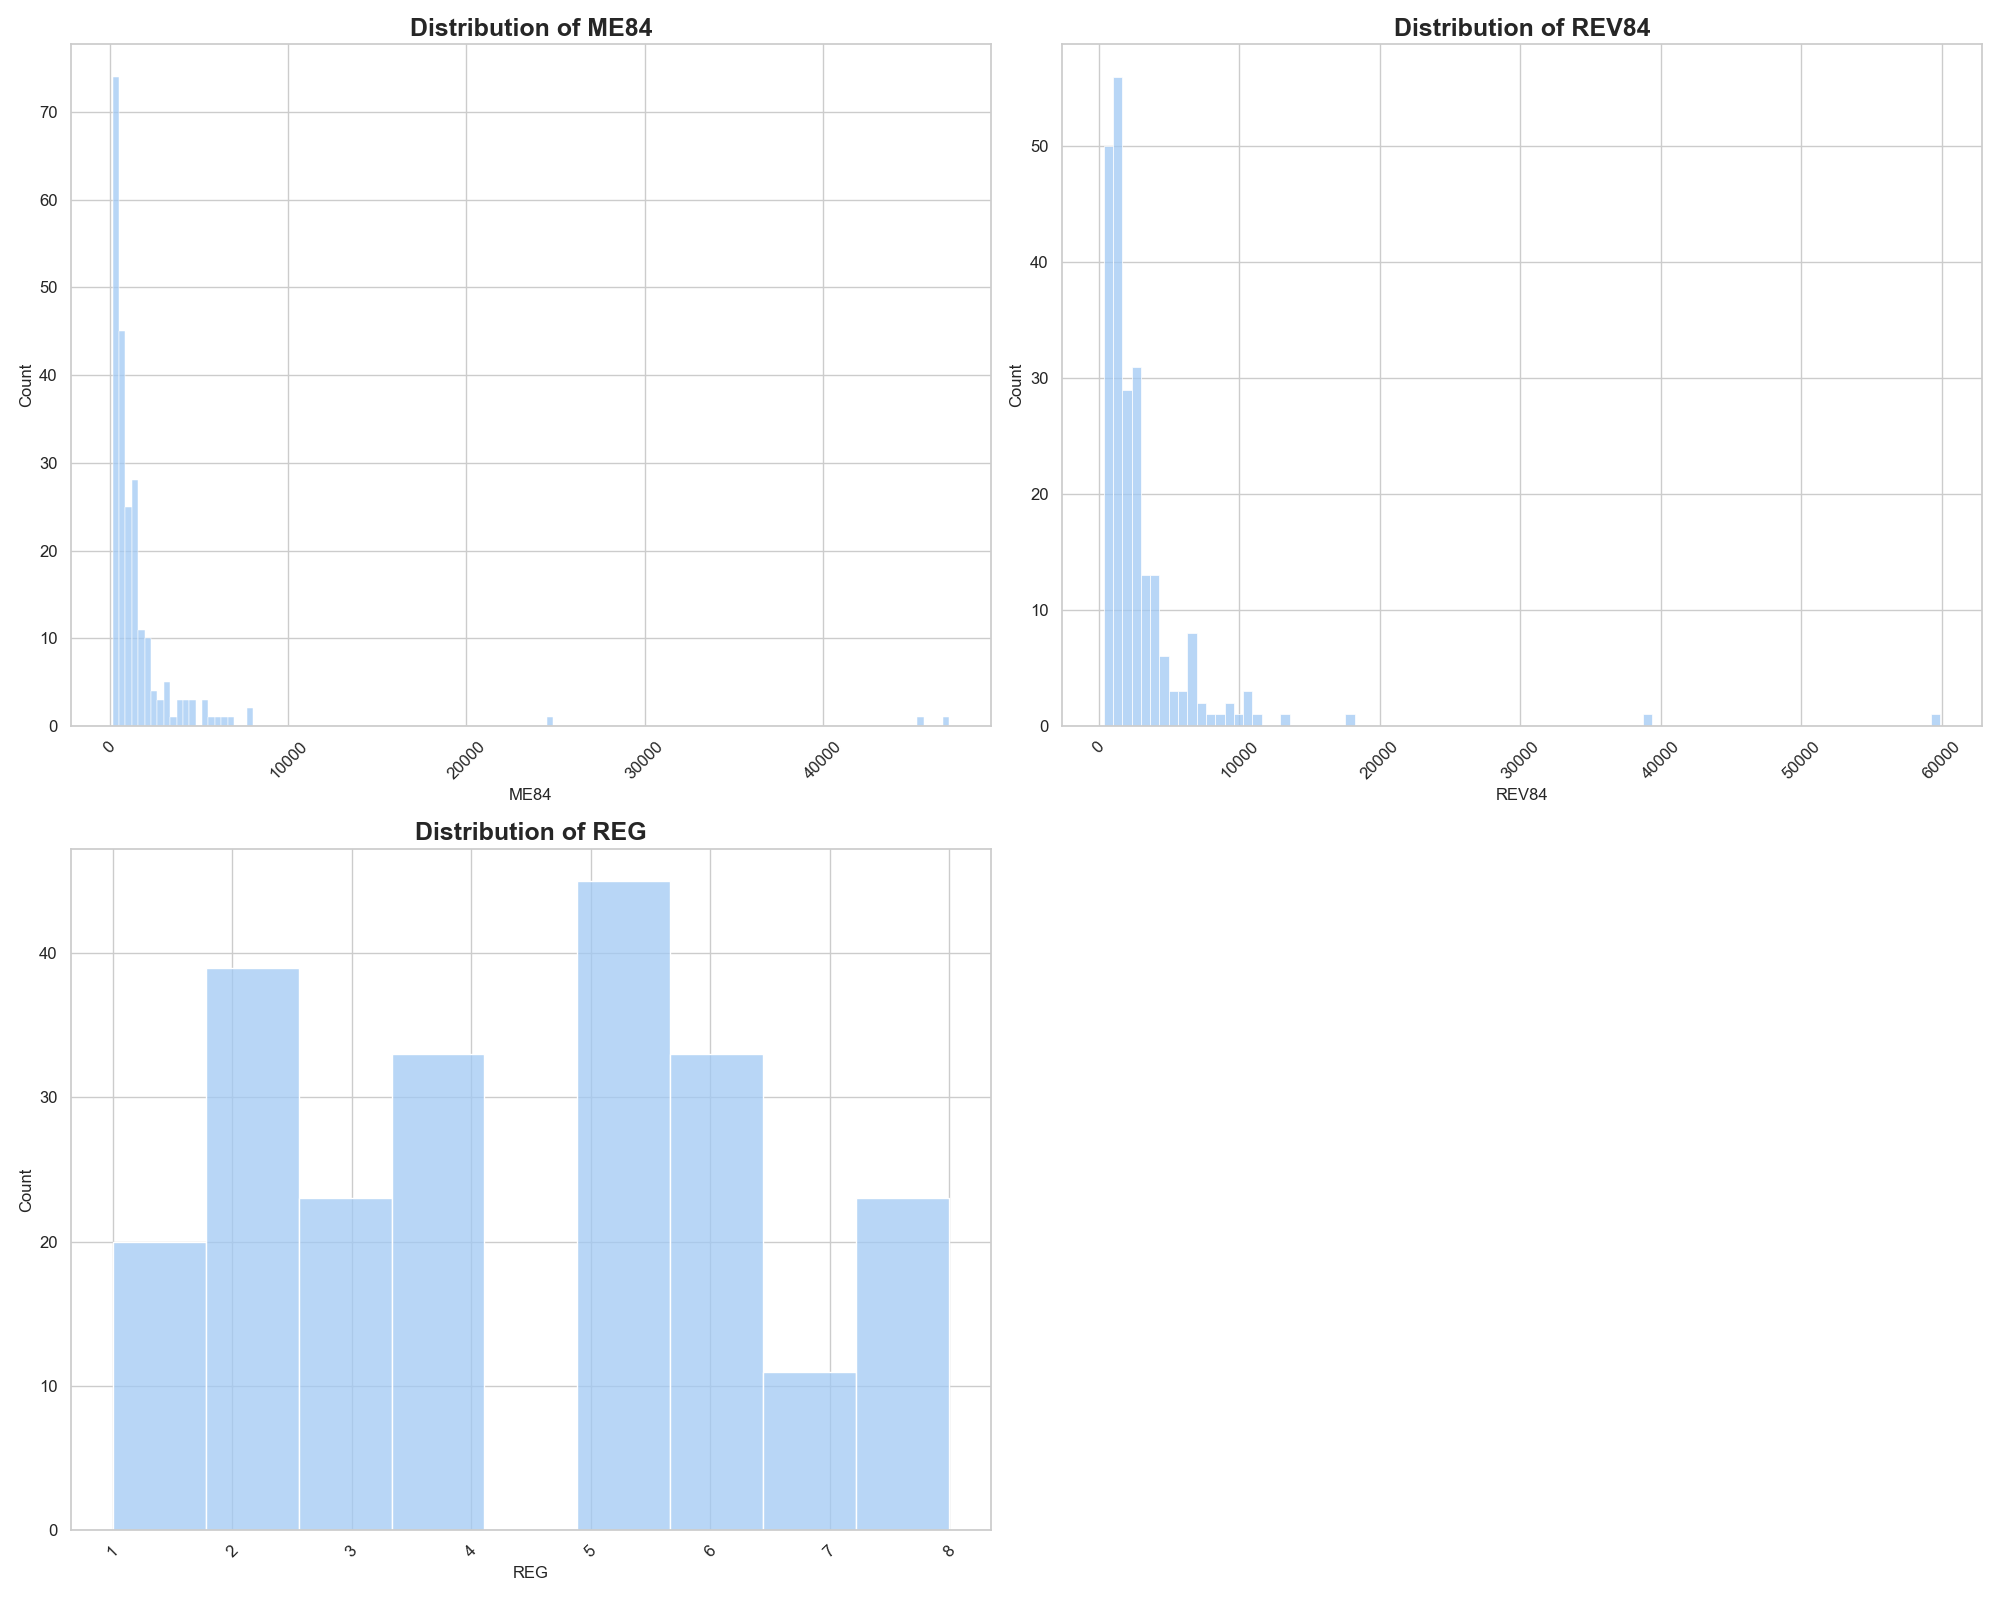
\includegraphics[width=0.9\textwidth]{/Users/julia/Desktop/semestr-5/automl/AutoPrep/examples/raport/raport/charts/numerical_distribution_page_2.png}%
\caption{Numerical Features Distribution {-} Page 2}%
\label{Numerical Features Distribution - Page 2}%
\end{figure}

%
Figure~\ref{Correlation heatmap.} %
 shows the correlation between features.%


\begin{figure}[H]%
\centering%
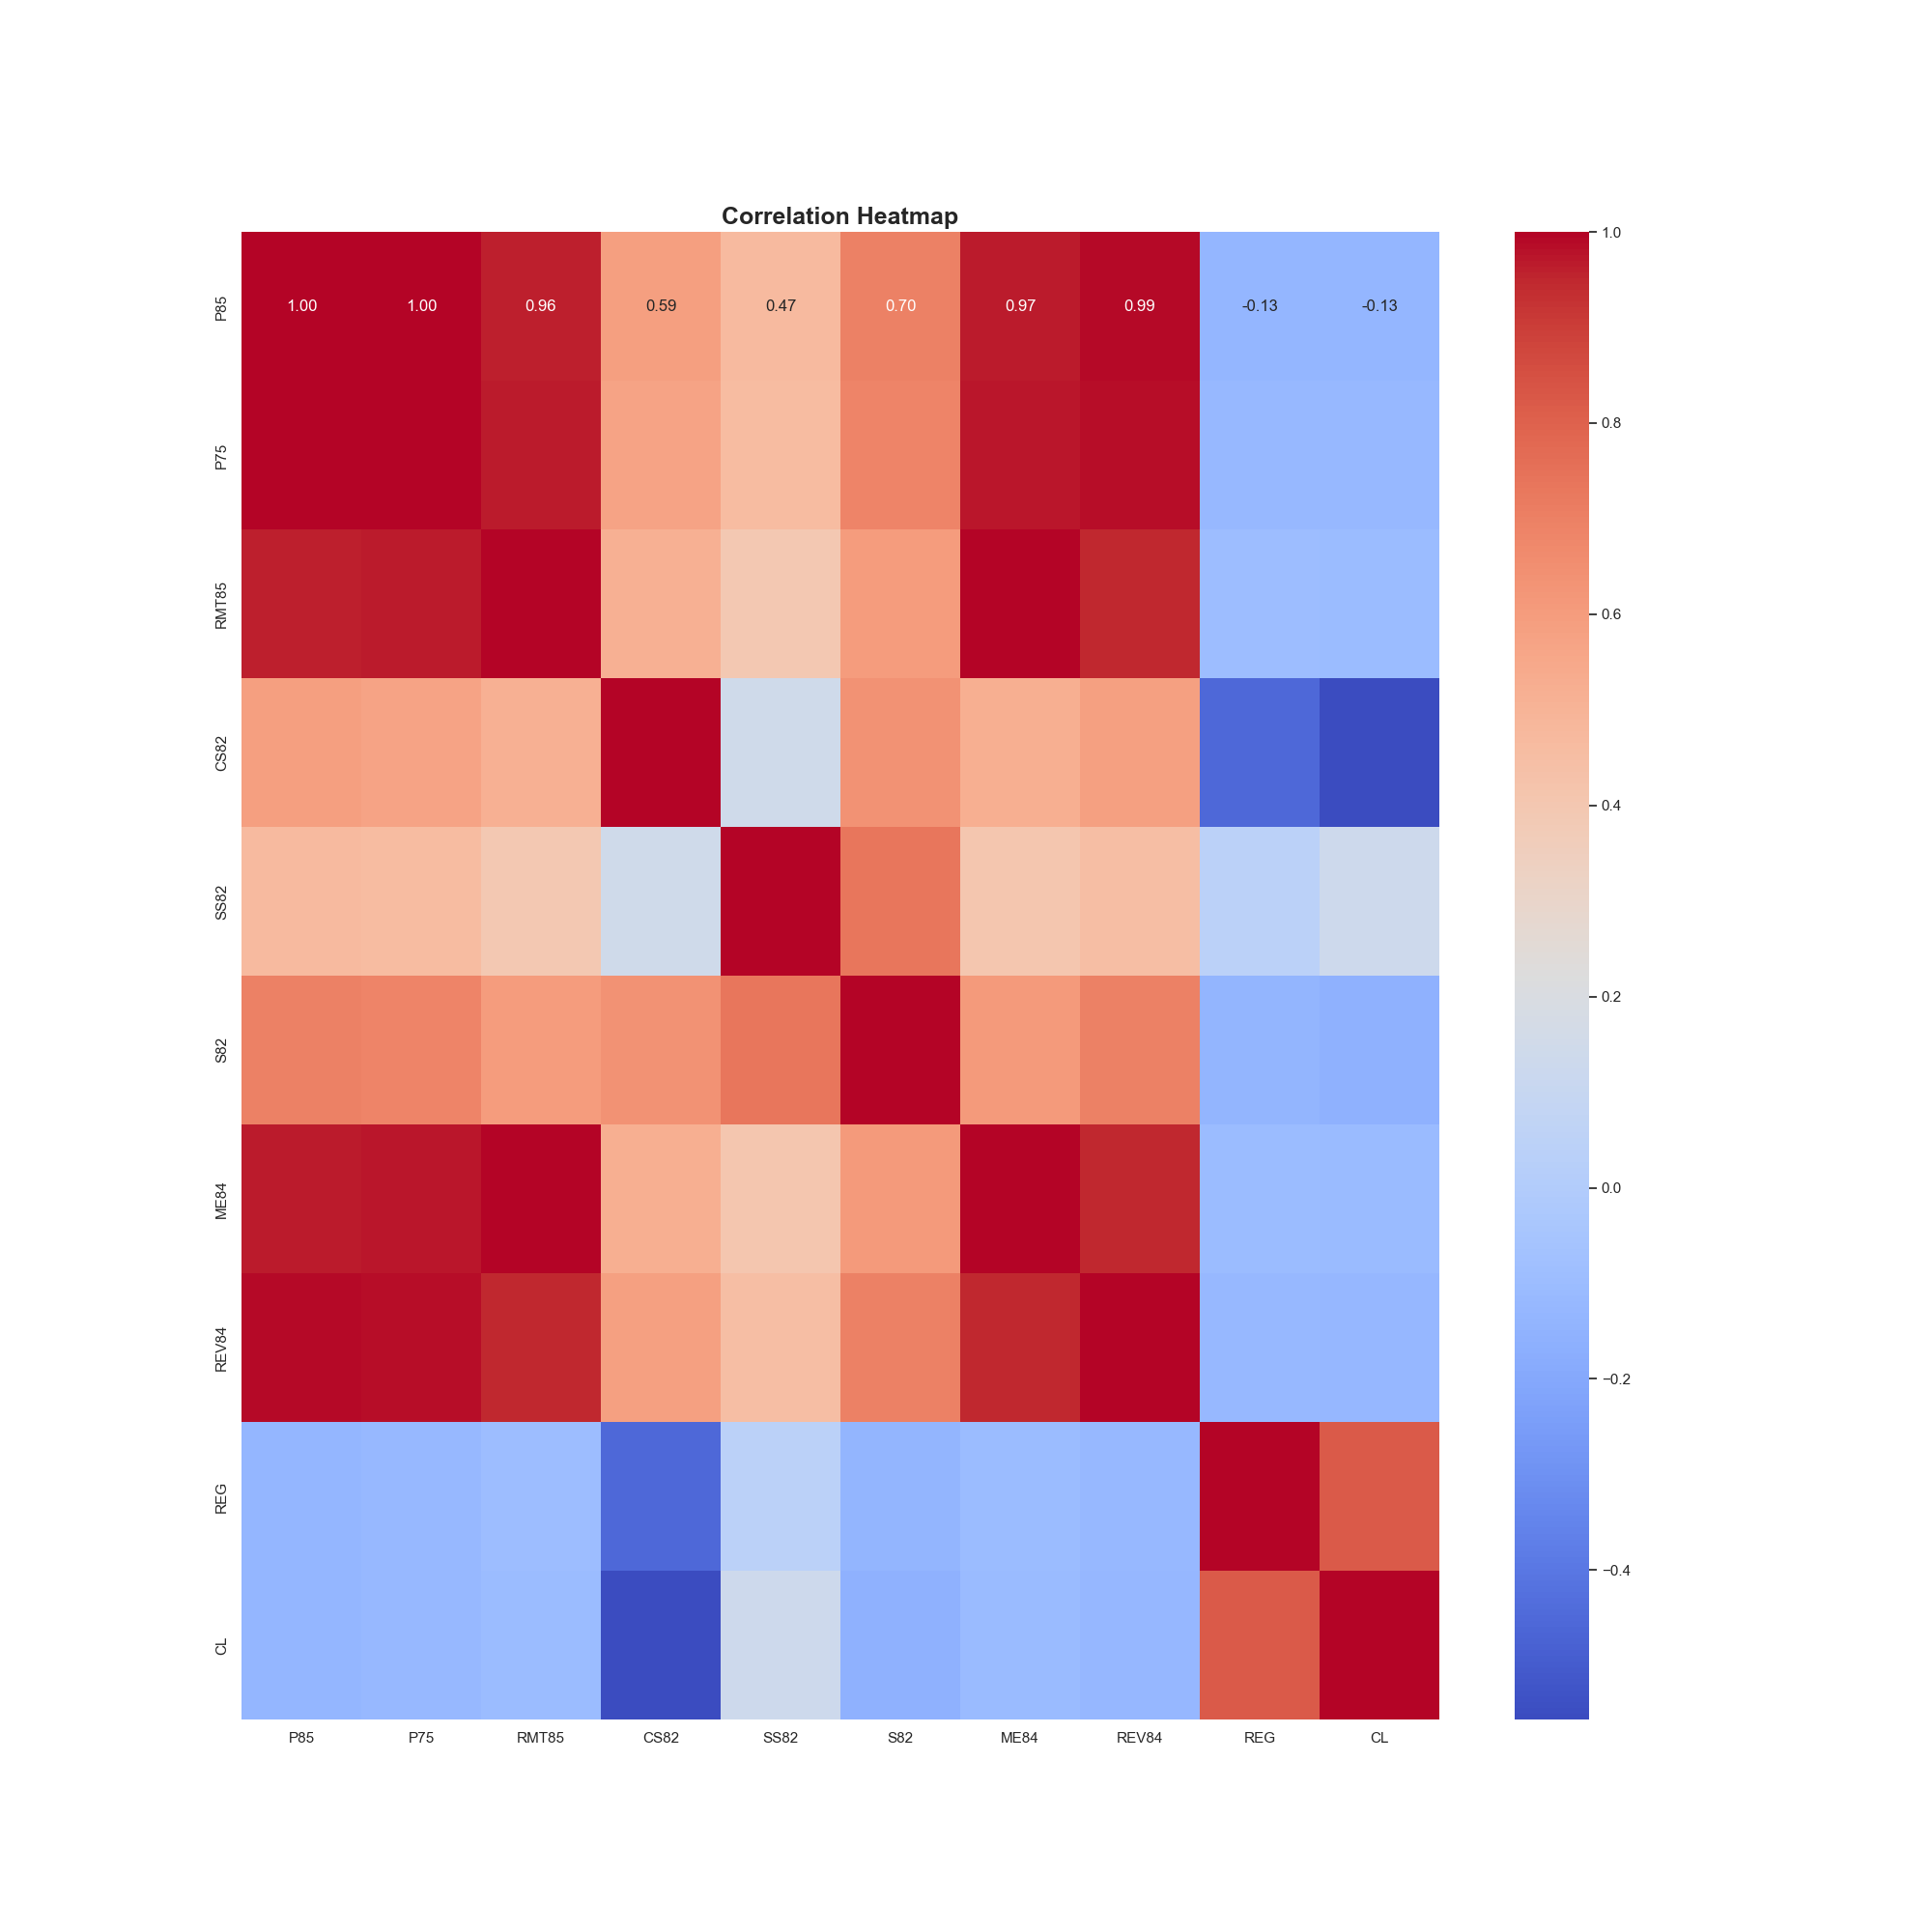
\includegraphics[width=0.9\textwidth]{/Users/julia/Desktop/semestr-5/automl/AutoPrep/examples/raport/raport/charts/correlation_heatmap.png}%
\caption{Correlation heatmap.}%
\label{Correlation heatmap.}%
\end{figure}

%
The boxplot of numerical features is presented on chart(s) below.%


\begin{figure}[H]%
\centering%
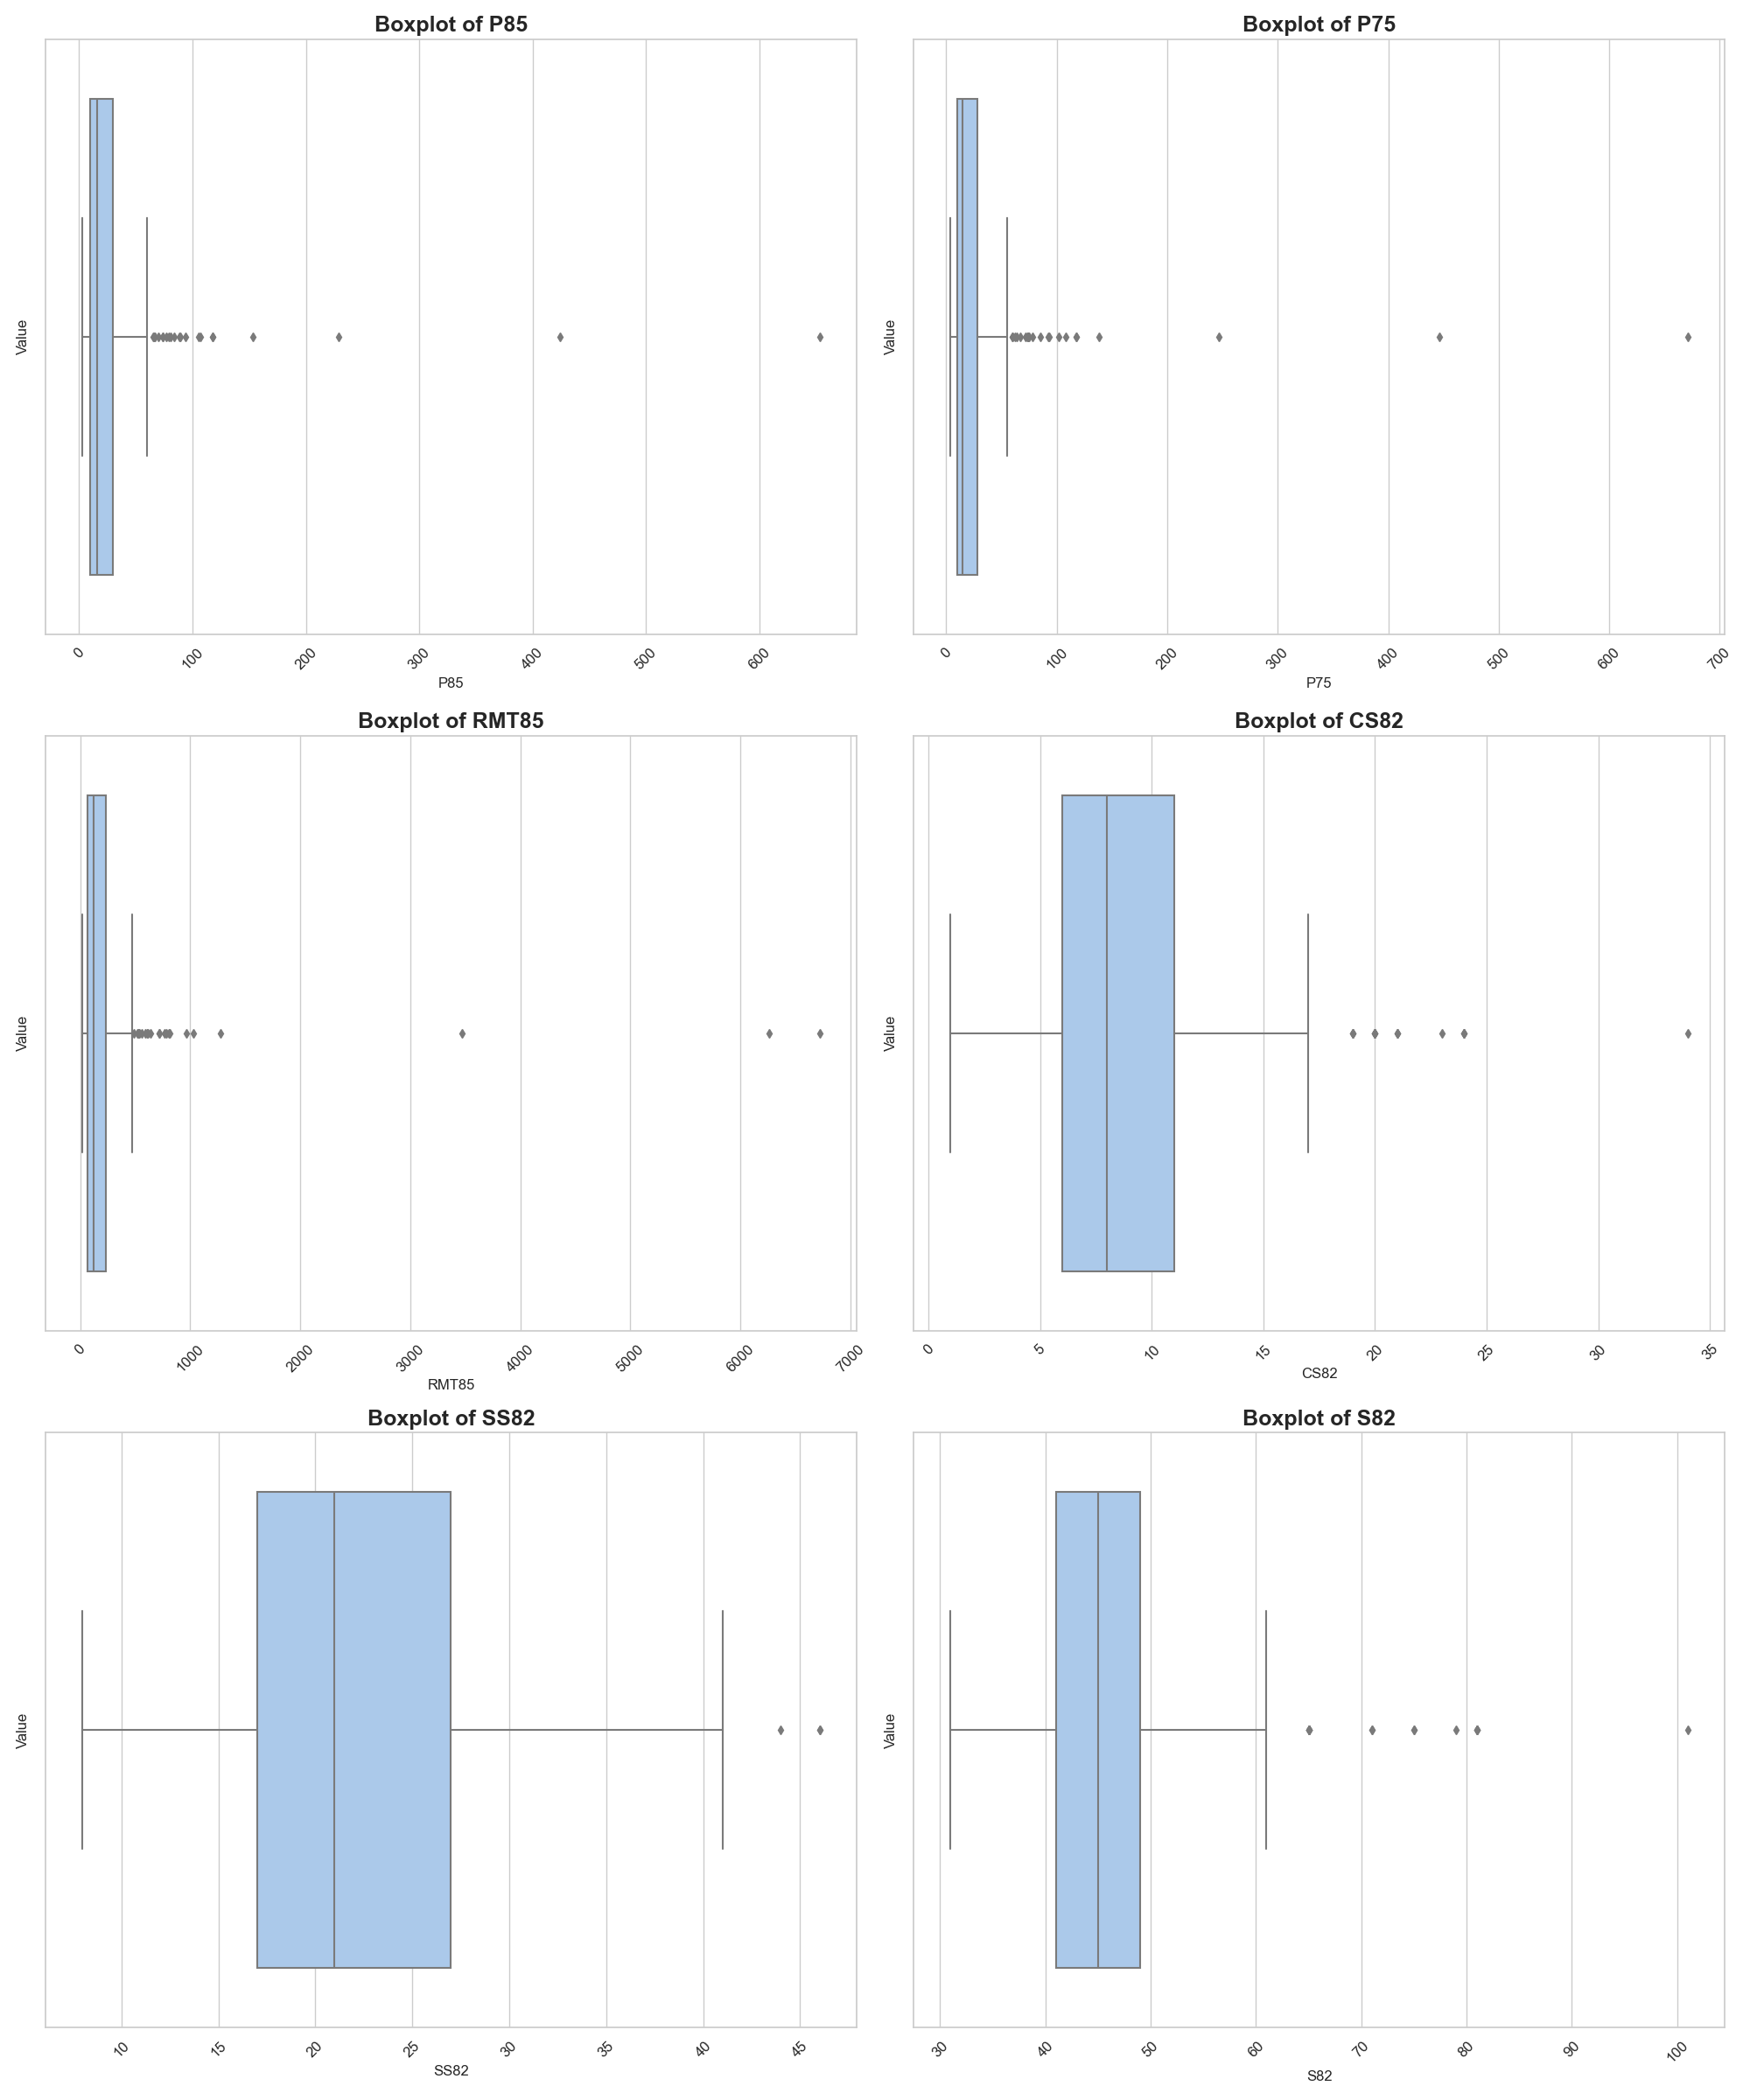
\includegraphics[width=0.9\textwidth]{/Users/julia/Desktop/semestr-5/automl/AutoPrep/examples/raport/raport/charts/boxplot_page_1.png}%
\caption{Boxplot page 1}%
\label{Boxplot page 1}%
\end{figure}

%


\begin{figure}[H]%
\centering%
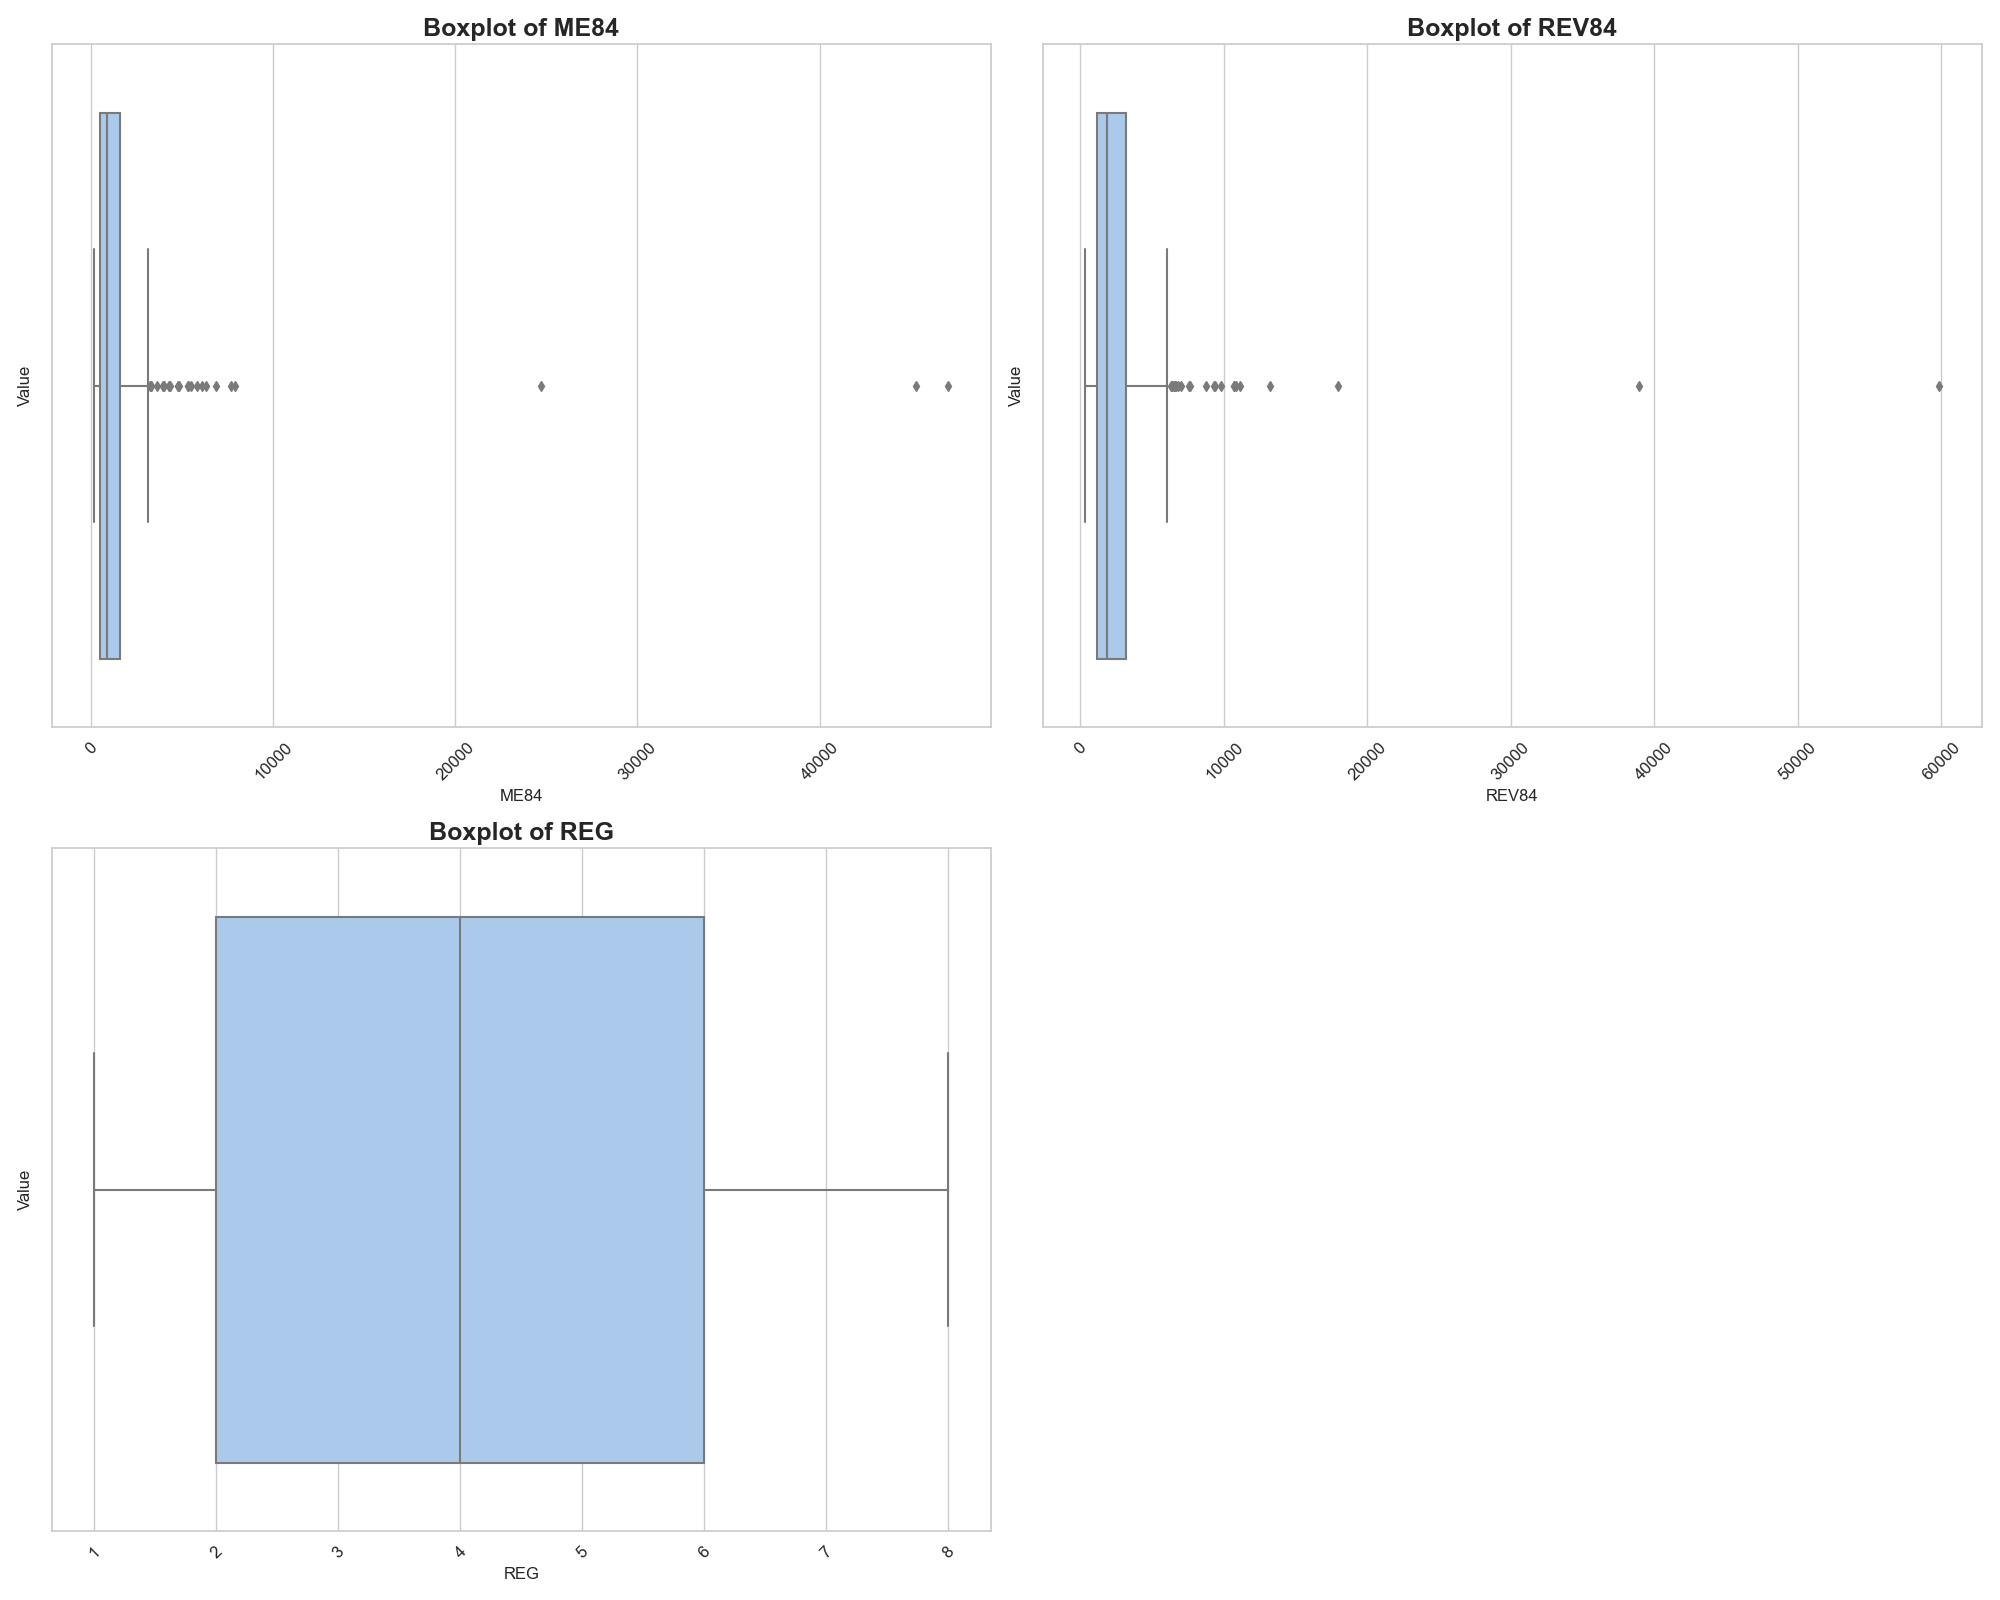
\includegraphics[width=0.9\textwidth]{/Users/julia/Desktop/semestr-5/automl/AutoPrep/examples/raport/raport/charts/boxplot_page_2.png}%
\caption{Boxplot page 2}%
\label{Boxplot page 2}%
\end{figure}

%
\section{Preprocessing}%
\label{sec:Preprocessing}%

%
This part of the report presents the results of the preprocessing process. It contains required, as well as non required, steps listed below. 
%
\\ \text{Required preprocessing steps}%
\begin{itemize}%
\item%
Missing data imputation%
\item%
Removing columns with 100\% unique categorical values%
\item%
Categorical features encoding%
\item%
Scaling%
\item%
Removing columns with 0 variance%
\item%
Detecting highly correlatd features%
\end{itemize}%
\\ \text{Additional preprocessing steps}%
\begin{itemize}%
\item%
Feature selection methods : Correlation with the target or Random Forest feature importance%
\item%
Dimention reduction techniques: PCA, VIF, UMAP%
\end{itemize}%
Preprocessing process was configured to select up to 3 best unique preprocessing pipelines. Pipelines were scored based on a simple model. Tables below show detailed description of the best pipelines as well as all step combinations that were examined. 
%


\begin{table}[H]%
\begin{center}%
\renewcommand{\arraystretch}{1.5}%
\begin{tabular}{p{20mm} p{160mm}}%
\hline%
\textbf{index}&\textbf{steps}\\%
\hline%
0&NAImputer, UniqueFilter, ColumnEncoder, VarianceFilter, CorrelationFilter, ColumnScaler\\%
\hline%
\end{tabular}%
\end{center}%
\caption{Pipelines steps overview.}%
\label{tab:pipelines_steps_overview}%
\end{table}

%


\begin{table}[H]%
\begin{center}%
\renewcommand{\arraystretch}{1.5}%
\begin{tabular}{l l l l l}%
\hline%
\textbf{score index}&\textbf{file name}&\textbf{score}&\textbf{fit duration}&\textbf{score duration}\\%
\hline%
0&preprocessing\_pipeline\_0.joblib&31.85&a moment&a moment\\%
1&preprocessing\_pipeline\_1.joblib&31.82&a moment&a moment\\%
2&preprocessing\_pipeline\_2.joblib&31.68&a moment&a moment\\%
\hline%
\end{tabular}%
\end{center}%
\caption{Best preprocessing pipelines.}%
\end{table}

%


\begin{table}[H]%
\begin{center}%
\renewcommand{\arraystretch}{1.5}%
\begin{tabular}{p{7mm} p{35mm} p{80mm} p{50mm}}%
\hline%
\textbf{step}&\textbf{name}&\textbf{description}&\textbf{params}\\%
\hline%
0&NAImputer&Imputes missing data.&\{"numeric\_imputer": "median", "categorical\_imputer": "most\_frequent"\}\\%
1&UniqueFilter&Removes categorical columns with 100\% unique values. Dropped columns: {[}{]}&\{\}\\%
2&ColumnEncoder&Encodes categorical columns using OneHotEncoder (for columns with <5 unique values) or TolerantLabelEncoder (for columns with >=5 unique values). Encodes target variable using LabelEncoder if provided.&\{\}\\%
3&VarianceFilter&Removes columns with zero variance. Dropped columns: {[}{]}&\{\}\\%
4&CorrelationFilter&Removes one column from pairs of columns correlated above correlation threshold: 0.8.&\{\}\\%
5&ColumnScaler&Scales numerical columns using one of 3 scaling methods.&\{"method": "minmax"\}\\%
\hline%
\end{tabular}%
\end{center}%
\caption{Best pipeline No. 0: steps overview.}%
\end{table}

%


\begin{table}[H]%
\begin{center}%
\renewcommand{\arraystretch}{1.5}%
\begin{tabular}{l l l l l l l l l}%
\hline%
\textbf{index}&\textbf{count}&\textbf{mean}&\textbf{std}&\textbf{min}&\textbf{25\%}&\textbf{50\%}&\textbf{75\%}&\textbf{max}\\%
\hline%
P85&227.00&{-}0.00&1.00&{-}0.48&{-}0.36&{-}0.25&0.00&11.12\\%
CS82&227.00&0.00&1.00&{-}1.64&{-}0.64&{-}0.24&0.37&4.99\\%
SS82&227.00&0.00&1.00&{-}1.93&{-}0.69&{-}0.13&0.70&3.33\\%
S82&227.00&{-}0.00&1.00&{-}1.53&{-}0.58&{-}0.20&0.18&5.11\\%
REG&227.00&{-}0.00&1.00&{-}1.60&{-}1.12&{-}0.16&0.80&1.77\\%
\hline%
\end{tabular}%
\end{center}%
\caption{Best pipeline No. 0: Output overview.}%
\end{table}

%


\begin{table}[H]%
\begin{center}%
\renewcommand{\arraystretch}{1.5}%
\begin{tabular}{p{7mm} p{35mm} p{80mm} p{50mm}}%
\hline%
\textbf{step}&\textbf{name}&\textbf{description}&\textbf{params}\\%
\hline%
0&NAImputer&Imputes missing data.&\{"numeric\_imputer": "median", "categorical\_imputer": "most\_frequent"\}\\%
1&UniqueFilter&Removes categorical columns with 100\% unique values. Dropped columns: {[}{]}&\{\}\\%
2&ColumnEncoder&Encodes categorical columns using OneHotEncoder (for columns with <5 unique values) or TolerantLabelEncoder (for columns with >=5 unique values). Encodes target variable using LabelEncoder if provided.&\{\}\\%
3&VarianceFilter&Removes columns with zero variance. Dropped columns: {[}{]}&\{\}\\%
4&CorrelationFilter&Removes one column from pairs of columns correlated above correlation threshold: 0.8.&\{\}\\%
5&ColumnScaler&Scales numerical columns using one of 3 scaling methods.&\{"method": "robust"\}\\%
\hline%
\end{tabular}%
\end{center}%
\caption{Best pipeline No. 1: steps overview.}%
\end{table}

%


\begin{table}[H]%
\begin{center}%
\renewcommand{\arraystretch}{1.5}%
\begin{tabular}{l l l l l l l l l}%
\hline%
\textbf{index}&\textbf{count}&\textbf{mean}&\textbf{std}&\textbf{min}&\textbf{25\%}&\textbf{50\%}&\textbf{75\%}&\textbf{max}\\%
\hline%
P85&227.00&0.04&0.09&0.00&0.01&0.02&0.04&1.00\\%
CS82&227.00&0.25&0.15&0.00&0.15&0.21&0.30&1.00\\%
SS82&227.00&0.37&0.19&0.00&0.24&0.34&0.50&1.00\\%
S82&227.00&0.23&0.15&0.00&0.14&0.20&0.26&1.00\\%
REG&227.00&0.48&0.30&0.00&0.14&0.43&0.71&1.00\\%
\hline%
\end{tabular}%
\end{center}%
\caption{Best pipeline No. 1: Output overview.}%
\end{table}

%


\begin{table}[H]%
\begin{center}%
\renewcommand{\arraystretch}{1.5}%
\begin{tabular}{p{7mm} p{35mm} p{80mm} p{50mm}}%
\hline%
\textbf{step}&\textbf{name}&\textbf{description}&\textbf{params}\\%
\hline%
0&NAImputer&Imputes missing data.&\{"numeric\_imputer": "median", "categorical\_imputer": "most\_frequent"\}\\%
1&UniqueFilter&Removes categorical columns with 100\% unique values. Dropped columns: {[}{]}&\{\}\\%
2&ColumnEncoder&Encodes categorical columns using OneHotEncoder (for columns with <5 unique values) or TolerantLabelEncoder (for columns with >=5 unique values). Encodes target variable using LabelEncoder if provided.&\{\}\\%
3&VarianceFilter&Removes columns with zero variance. Dropped columns: {[}{]}&\{\}\\%
4&CorrelationFilter&Removes one column from pairs of columns correlated above correlation threshold: 0.8.&\{\}\\%
5&ColumnScaler&Scales numerical columns using one of 3 scaling methods.&\{"method": "standard"\}\\%
\hline%
\end{tabular}%
\end{center}%
\caption{Best pipeline No. 2: steps overview.}%
\end{table}

%


\begin{table}[H]%
\begin{center}%
\renewcommand{\arraystretch}{1.5}%
\begin{tabular}{l l l l l l l l l}%
\hline%
\textbf{index}&\textbf{count}&\textbf{mean}&\textbf{std}&\textbf{min}&\textbf{25\%}&\textbf{50\%}&\textbf{75\%}&\textbf{max}\\%
\hline%
P85&227.00&0.70&2.81&{-}0.65&{-}0.30&0.00&0.70&31.85\\%
CS82&227.00&0.24&1.00&{-}1.40&{-}0.40&0.00&0.60&5.20\\%
SS82&227.00&0.10&0.72&{-}1.30&{-}0.40&0.00&0.60&2.50\\%
S82&227.00&0.27&1.32&{-}1.75&{-}0.50&0.00&0.50&7.00\\%
REG&227.00&0.08&0.52&{-}0.75&{-}0.50&0.00&0.50&1.00\\%
\hline%
\end{tabular}%
\end{center}%
\caption{Best pipeline No. 2: Output overview.}%
\end{table}

%
You may also find all pipelines' runtime statistic in %
Table~\ref{tab:preprocessing_pipelines_runtime_statistics}%


\begin{table}[H]%
\begin{center}%
\renewcommand{\arraystretch}{1.5}%
\begin{tabular}{l l}%
\hline%
\textbf{Category}&\textbf{Value}\\%
\hline%
Unique created pipelines&1\\%
All created pipelines (after exploading each step params)&3\\%
All pipelines fit time&2 seconds\\%
All pipelines score time&2 seconds\\%
scores\_count&3.00\\%
scores\_mean&31.78\\%
scores\_std&0.09\\%
scores\_min&31.68\\%
scores\_25\%&31.75\\%
scores\_50\%&31.82\\%
scores\_75\%&31.84\\%
scores\_max&31.85\\%
Scoring function&<class 'str'>\\%
Scoring model&RandomForestRegressor\\%
\hline%
\end{tabular}%
\end{center}%
\caption{Preprocessing pipelines runtime statistics.}%
\label{tab:preprocessing_pipelines_runtime_statistics}%
\end{table}

%
\section{Modeling}%
\label{sec:Modeling}%

%
\subsection{Overview}%
\label{subsec:Overview}%

%
This part of the report presents the results of the modeling process. There were regression 6 models trained for each of the best preprocessing pipelines.%
The following models were used in the modeling process.%
\begin{itemize}%
\item%
LinearSVR%
\item%
KNeighborsRegressor%
\item%
RandomForestRegressor%
\item%
BayesianRidge%
\item%
GradientBoostingRegressor%
\item%
LinearRegression%
\end{itemize}%
\subsection{Hyperparameter tuning}%
\label{subsec:Hyperparametertuning}%

%
This section presents the results of hyperparameter tuning for each of the best 3 models using RandomizedSearchCV. Param grids used for each model are presented in the tables below.%


\begin{table}[H]%
\begin{center}%
\renewcommand{\arraystretch}{1.5}%
\begin{tabular}{l l}%
\hline%
\textbf{Category}&\textbf{Value}\\%
\hline%
epsilon&{[}0.0, 0.1, 0.2, 0.5, 1.0{]}\\%
C&{[}0.1, 1.0, 10.0, 100.0{]}\\%
loss&{[}'epsilon\_insensitive', 'squared\_epsilon\_insensitive'{]}\\%
fit\_intercept&{[}True, False{]}\\%
\hline%
\end{tabular}%
\end{center}%
\caption{Param grid for model LinearSVR.}%
\end{table}

%


\begin{table}[H]%
\begin{center}%
\renewcommand{\arraystretch}{1.5}%
\begin{tabular}{l l}%
\hline%
\textbf{Category}&\textbf{Value}\\%
\hline%
n\_neighbors&{[}5, 10, 15{]}\\%
weights&{[}'uniform', 'distance'{]}\\%
algorithm&{[}'auto', 'ball\_tree', 'kd\_tree', 'brute'{]}\\%
leaf\_size&{[}30, 40, 50{]}\\%
p&{[}1, 2{]}\\%
\hline%
\end{tabular}%
\end{center}%
\caption{Param grid for model KNeighboursRegressor.}%
\end{table}

%


\begin{table}[H]%
\begin{center}%
\renewcommand{\arraystretch}{1.5}%
\begin{tabular}{l l}%
\hline%
\textbf{Category}&\textbf{Value}\\%
\hline%
n\_estimators&{[}100, 200, 300{]}\\%
max\_depth&{[}None, 5, 10, 15, 20{]}\\%
min\_samples\_split&{[}2, 5, 10{]}\\%
min\_samples\_leaf&{[}1, 2, 4{]}\\%
max\_features&{[}'sqrt', 'log2', None{]}\\%
bootstrap&{[}True, False{]}\\%
random\_state&{[}42{]}\\%
\hline%
\end{tabular}%
\end{center}%
\caption{Param grid for model RandomForestRegressor.}%
\end{table}

%


\begin{table}[H]%
\begin{center}%
\renewcommand{\arraystretch}{1.5}%
\begin{tabular}{l l}%
\hline%
\textbf{Category}&\textbf{Value}\\%
\hline%
max\_iter&{[}300, 400, 500{]}\\%
tol&{[}0.001, 0.0001, 1e{-}05{]}\\%
alpha\_1&{[}1e{-}06, 1e{-}07, 1e{-}08{]}\\%
alpha\_2&{[}1e{-}06, 1e{-}07, 1e{-}08{]}\\%
lambda\_1&{[}1e{-}06, 1e{-}07, 1e{-}08{]}\\%
lambda\_2&{[}1e{-}06, 1e{-}07, 1e{-}08{]}\\%
\hline%
\end{tabular}%
\end{center}%
\caption{Param grid for model BayesianRidgeRegressor.}%
\end{table}

%


\begin{table}[H]%
\begin{center}%
\renewcommand{\arraystretch}{1.5}%
\begin{tabular}{l l}%
\hline%
\textbf{Category}&\textbf{Value}\\%
\hline%
n\_estimators&{[}100, 200, 300{]}\\%
learning\_rate&{[}0.1, 0.05, 0.02{]}\\%
max\_depth&{[}4, 6, 8{]}\\%
min\_samples\_split&{[}2, 5, 10{]}\\%
min\_samples\_leaf&{[}1, 2, 4{]}\\%
subsample&{[}1.0, 0.5{]}\\%
random\_state&{[}42{]}\\%
\hline%
\end{tabular}%
\end{center}%
\caption{Param grid for model GradientBoostingRegressor.}%
\end{table}

%


\begin{table}[H]%
\begin{center}%
\renewcommand{\arraystretch}{1.5}%
\begin{tabular}{l l}%
\hline%
\textbf{Category}&\textbf{Value}\\%
\hline%
fit\_intercept&{[}True, False{]}\\%
\hline%
\end{tabular}%
\end{center}%
\caption{Param grid for model LinearRegression.}%
\end{table}

%
Table~\ref{tab:best_models_results} %
presents the best models and pipelines along with their hyperparameters, mean fit time, and test score.%


\begin{table}[H]%
\begin{center}%
\renewcommand{\arraystretch}{1.5}%
\begin{tabular}{p{35mm} p{35mm} p{45mm} p{25mm} p{15mm}}%
\hline%
\textbf{Model}&\textbf{Pipeline}&\textbf{Best params}&\textbf{Mean fit time}&\textbf{Test score}\\%
\hline%
LinearSVR&final\_pipeline\_0.joblib&\{"loss": "epsilon\_insensitive", "fit\_intercept": false, "epsilon": 0.2, "C": 1.0\}&0.00&71.53\\%
LinearSVR&final\_pipeline\_2.joblib&\{"loss": "epsilon\_insensitive", "fit\_intercept": false, "epsilon": 0.0, "C": 1.0\}&0.00&72.54\\%
LinearSVR&final\_pipeline\_1.joblib&\{"loss": "epsilon\_insensitive", "fit\_intercept": true, "epsilon": 0.0, "C": 0.1\}&0.00&250.06\\%
\hline%
\end{tabular}%
\end{center}%
\caption{Best models results}%
\label{tab:best_models_results}%
\end{table}

%
\end{document}